\documentclass[aip,jmp,reprint,onecolumn,nofootinbib]{revtex4-2}

\usepackage{amsmath,amssymb,amsfonts}
\usepackage{graphicx}
\usepackage{bm}
\usepackage{hyperref}

\begin{document}

\title{Dynamic Entity Field Integration (DEFI): A Coupled Lagrangian Construction Unifying SEFI Identity and GWFM Geometry}

\author{Jason Dutton}
\affiliation{Castlewood, Virginia, USA}

\date{2026}

\begin{abstract}
Dynamic Entity Field Integration (DEFI) has appeared throughout the SEFI/GWFM
literature as the unifying field law binding the Single Entity Field Interpretation
(SEFI) identity layer to the Geometric Worldline Field Model (GWFM) geometry
layer, expressed through the invariance condition
$\frac{D}{d\tau}(\kappa,\tau_g,\dot I^a,\ddot I^a)=0$ on a stability manifold $\Sigma$.
This condition has to date been stipulated rather than derived, a gap noted
explicitly in the Limitations of the unified geometric field theory. This paper
supplies the missing construction. DEFI is defined as a joint Lagrangian dynamical
system on $M\times\mathcal{I}$, with a fully symmetric coupling potential linking
GWFM curvature/torsion invariants to SEFI's Sovereignty and Warp identity
coordinates, weighted by the Authorship coordinate. The stipulated invariance
condition is recovered as the equilibrium condition of this coupled system rather
than assumed. A conserved Origin charge is derived via Noether's theorem for the
decoupled Origin sector. This construction requires an explicit extension of SEFI,
promoting its originally scalar identity functional $F=O+A+S+W$ to a four-vector
$I^a=(I_O,I_A,I_S,I_W)$ on an identity-space manifold $\mathcal{I}=\mathbb{R}^4$,
which is stated here as a deliberate axiomatic extension rather than a silent
reinterpretation.
\end{abstract}

\maketitle

\section{Introduction}

Across the SEFI/GWFM literature, Dynamic Entity Field Integration (DEFI) is
invoked as ``the unifying field law that binds SEFI identity and GWFM geometry
into a single stability surface'' \cite{DuttonSEFI2026,DuttonElectronField2026},
and its only concrete mathematical content is the stipulated dynamical invariance
condition
\begin{equation}
\frac{D}{d\tau}\left(\kappa,\ \tau_g,\ \dot I^a,\ \ddot I^a\right) = 0
\qquad \text{on } \Sigma,
\label{eq:stipulated}
\end{equation}
appearing in the unified geometric field theory \cite{DuttonUnified2026}. No prior
document derives Eq.~\eqref{eq:stipulated} from an action principle; it is asserted
as a definition of ideal evolution. The unified paper's own Limitations section
acknowledges this directly: ``the operator $T$ is phenomenological and not derived
from a variational principle.'' The present paper closes that gap by constructing
DEFI as a genuine coupled dynamical system whose equations of motion reproduce
Eq.~\eqref{eq:stipulated} as an equilibrium condition, rather than as an axiom.

\begin{figure}[tb]
 \centering 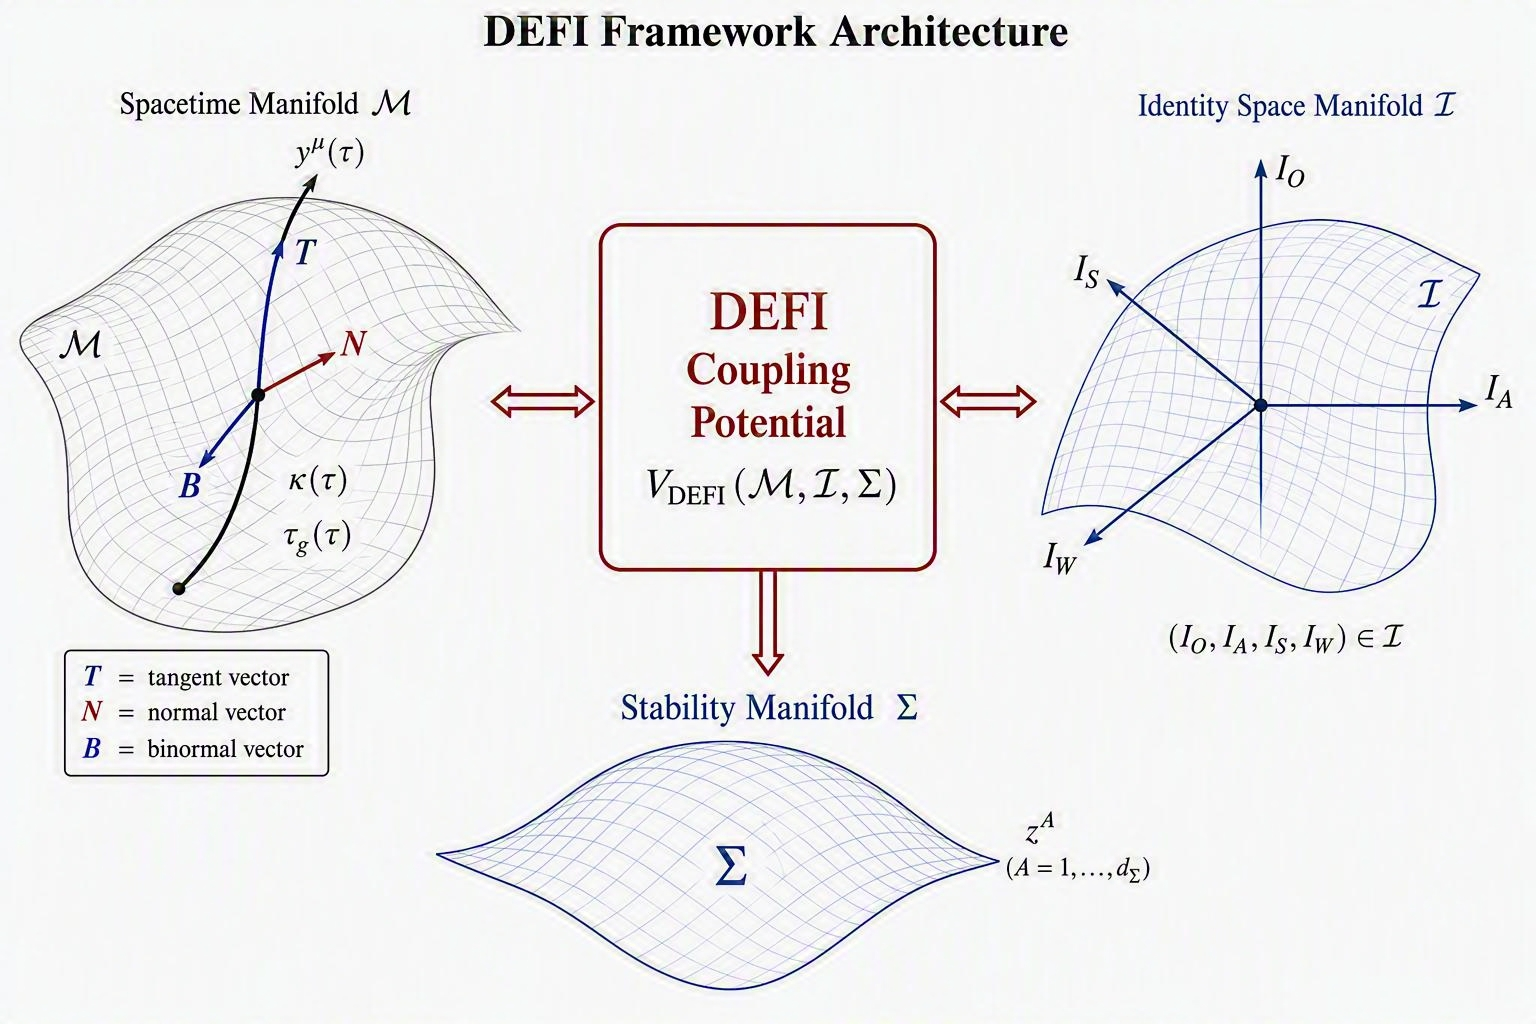
\includegraphics[width=0.90\textwidth]{fig1_defi_architecture.jpg}
 \caption{ Conceptual structure of DEFI as the variational bridge between SEFI identity-space dynamics and GWFM worldline geometry. The coupled DEFI framework generates the integrated consistency conditions that appear in the unified geometric field theory. }
 \label{fig:defi_architecture} \end{figure}
\subsection{A Required Extension of SEFI}

The original SEFI formal construction \cite{DuttonSEFI2026} defines field identity
as a \emph{scalar} functional,
\begin{equation}
F(t) = O(r(t)) + A(r(t),\kappa(t)) + S(r(t)) + W(r(t)),
\label{eq:sefi-scalar}
\end{equation}
summing the Origin, Authorship, Sovereignty, and Warp layers into a single number
evaluated along the worldline. The later unified paper \cite{DuttonUnified2026}
instead treats $I^a=(I_O,I_A,I_S,I_W)$ as coordinates on an identity-space manifold
$\mathcal{I}=\mathbb{R}^4$ with metric $g_I=\mathrm{diag}(\alpha,\beta,\gamma,\delta)$,
differentiable in $\tau$ as a four-vector. These are not the same mathematical
object: a scalar sum cannot be covariantly differentiated in four independent
directions, so Eq.~\eqref{eq:stipulated} is only well-defined under the
vector reading.

This paper adopts the vector reading explicitly, as a stated extension of SEFI
rather than a silent correction of the earlier scalar definition. We record this
as:

\begin{quote}
\textbf{DEFI Axiom 0 (Vectorization of Identity).} SEFI's scalar identity
functional $F=O+A+S+W$ is extended to a four-vector $I^a=(I_O,I_A,I_S,I_W)\in\mathcal{I}$
carrying an independent metric $g_I=\mathrm{diag}(\alpha,\beta,\gamma,\delta)$. The
original scalar $F$ is recovered as $F = \delta_{ab}\,\mathbf{1}^a I^b$, the
coordinate sum of the vector, so that Eq.~\eqref{eq:sefi-scalar} is a special
contraction of the DEFI-extended identity vector rather than a competing
definition.
\end{quote}

\section{Configuration Space}

DEFI is defined on the product space $M\times\mathcal{I}$, where $M$ is the
spacetime manifold carrying the GWFM worldline and $\mathcal{I}=\mathbb{R}^4$ is
the SEFI identity-space manifold of Axiom 0. A single trajectory
\begin{equation}
z(\tau) = \left(y^\mu(\tau),\ I^a(\tau)\right) \in M \times \mathcal{I}
\end{equation}

\begin{figure}[tb]
\centering 
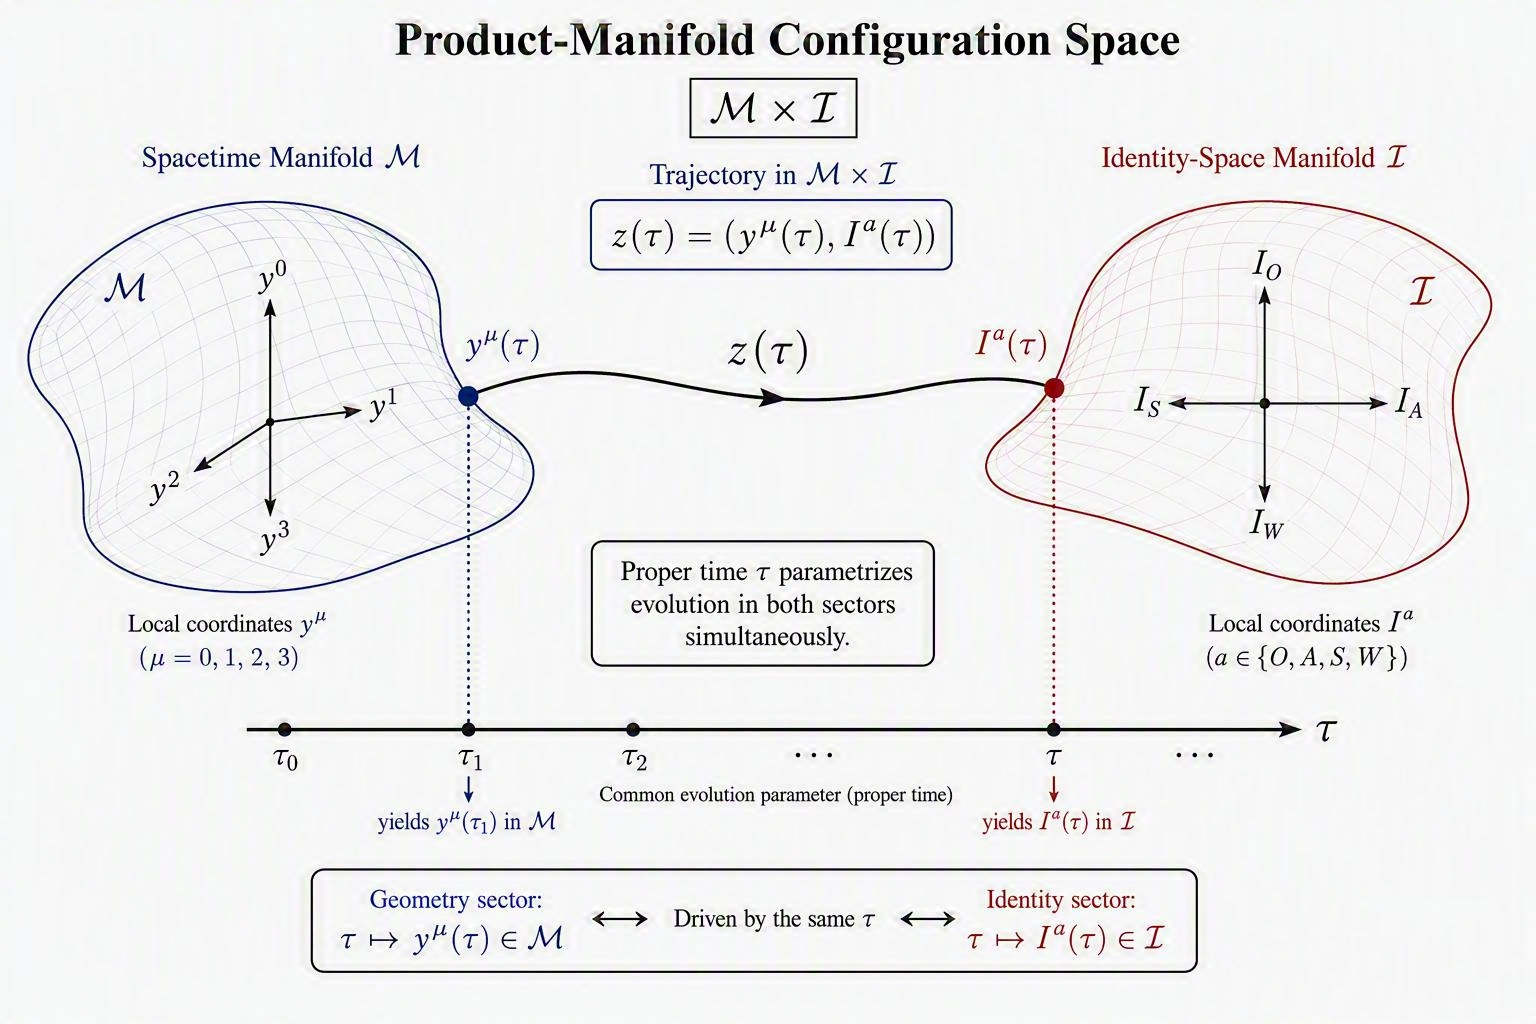
\includegraphics[width=0.95
\textwidth]{fig2_product_manifold.jpg}
 \caption{ Product-manifold configuration space $M
\times\mathcal{I}$. The trajectory $z(\tau)=\left(y^\mu(\tau),I^a(\tau)\right)$ evolves simultaneously through the spacetime manifold $M$ and the identity-space manifold $\mathcal{I}$ under a common proper-time parameter $\tau$. }
 \label{fig:product_manifold}
 \end{figure}

carries both sectors simultaneously in one proper-time parameter $\tau$. Geometric
invariants $\kappa(\tau),\tau_g(\tau)$ are defined through the Frenet--Serret frame
$(T,N,B)$ of $y(\tau)$ \cite{DoCarmo1976}, exactly as in GWFM \cite{DuttonElectronField2026}.

\section{Sector Lagrangians}

\subsection{Geometry Sector (GWFM, unchanged)}
\begin{equation}
L_{\text{geom}} = -m\sqrt{-g_{\mu\nu}(y)\,\dot y^\mu \dot y^\nu}.
\end{equation}

\subsection{Identity Sector}
\begin{equation}
L_{\text{ident}} = \frac{1}{2}g_I^{ab}\dot I_a \dot I_b
- \frac{1}{2}\left(\alpha I_O^2+\beta I_A^2+\gamma I_S^2+\delta I_W^2\right).
\end{equation}
Each identity coordinate is, in isolation, a harmonic oscillator in $\tau$, and the
four coordinates together form a system of coupled oscillators once
$U_{\text{DEFI}}$ is introduced below \cite{Strogatz2015}. This
gives SEFI's Origin-layer stability bound $\|\ddot r\|\le S_0$
\cite{DuttonSEFI2026} a dynamical origin: bounded oscillatory motion is now a
derived consequence of $L_{\text{ident}}$ rather than an externally imposed
inequality.

\section{The DEFI Coupling Potential}

\begin{figure}[tb]
 \centering 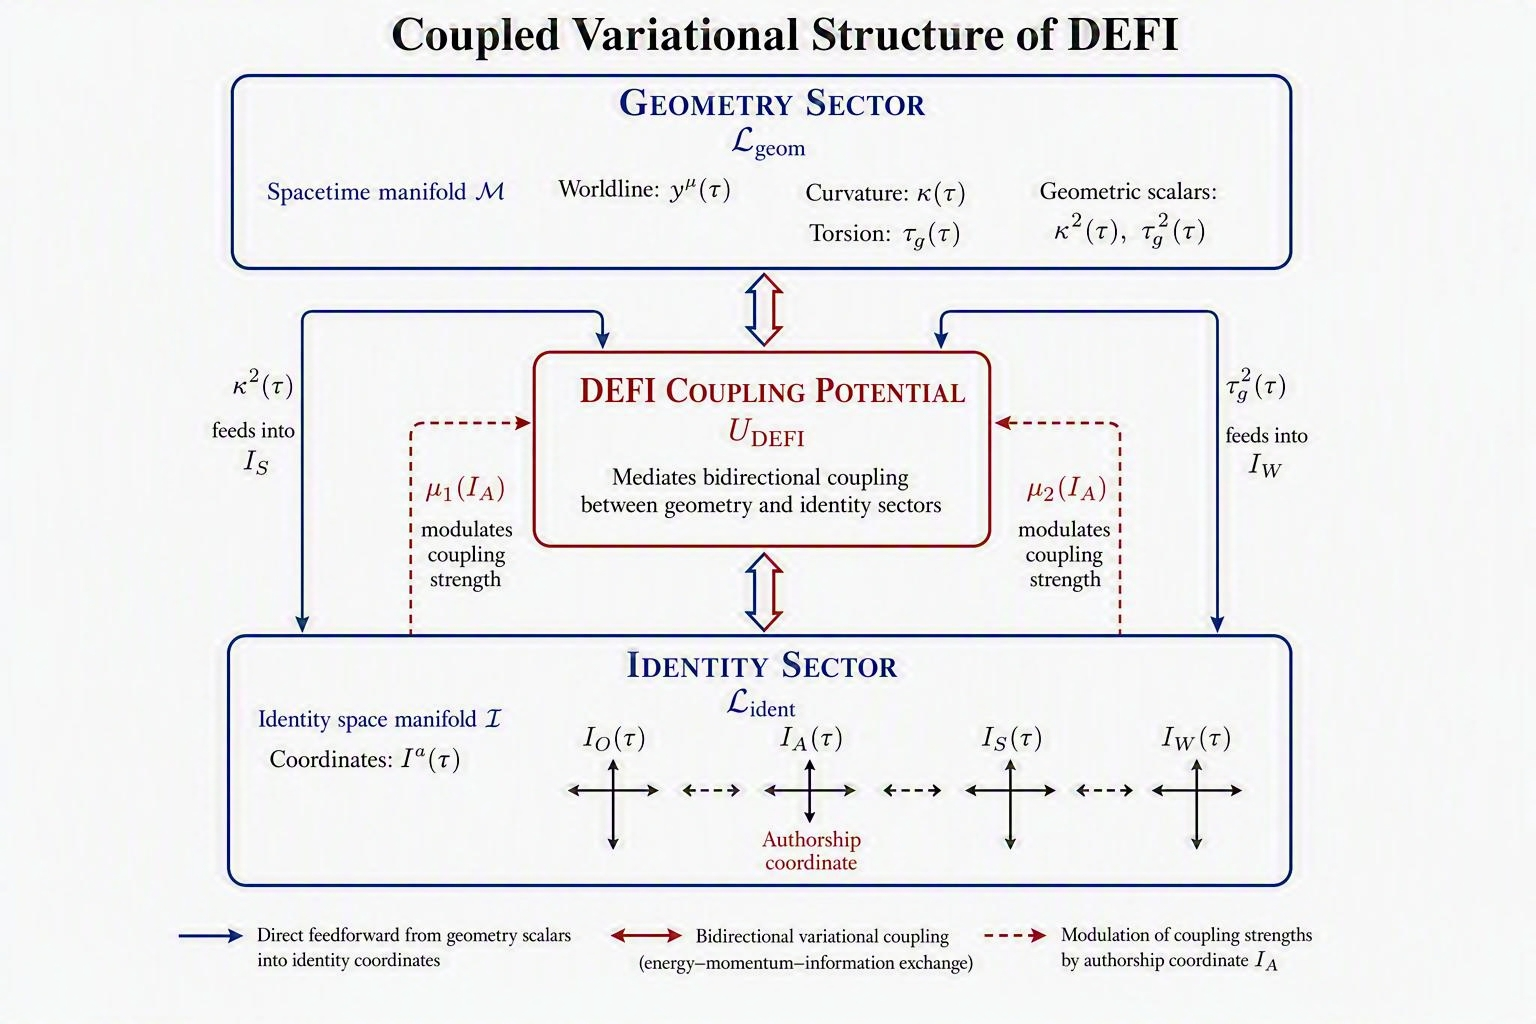
\includegraphics[width=0.95\textwidth]{fig3_variational_structure.jpg}
 \caption{ Variational structure of DEFI. The coupling potential mediates bidirectional interaction between GWFM geometry variables and SEFI identity variables, with authorship-dependent coupling strengths. } 
\label{fig:variational_structure}
 \end{figure}

The coupling potential is required to be fully symmetric: geometry acts on
identity and identity acts on geometry within a single stationary action, with
neither sector prior to the other. We propose
\begin{equation}
U_{\text{DEFI}}(\kappa,\tau_g,I^a) =
\mu_1(I_A)\,\kappa^2 I_S \;+\; \mu_2(I_A)\,\tau_g^2 I_W.
\label{eq:coupling}
\end{equation}

This pairing is not arbitrary; each term is fixed by the canonical SEFI layer
definitions \cite{DuttonSEFI2026}:
\begin{itemize}
\item \textbf{Sovereignty $\leftrightarrow$ curvature.} SEFI defines Sovereignty
through the stability/acceleration bound of Eq.~\eqref{eq:sefi-scalar}'s origin
condition; curvature $\kappa$ is GWFM's geometric measure of how sharply a
worldline accelerates. Pairing $I_S$ with $\kappa^2$ makes this correspondence
dynamical.
\item \textbf{Warp $\leftrightarrow$ torsion.} The SEFI paper states explicitly
that warp operators perform ``curvature modulation, torsion modulation''
\cite{DuttonSEFI2026}; torsion $\tau_g$ is GWFM's natural analogue of twisting
transformation. Pairing $I_W$ with $\tau_g^2$ follows directly.
\item \textbf{Authorship as coupling weight, not an additive term.} In the
original SEFI paper, Authorship is not its own geometric quantity but a weighted
sum $F_A=\sum_i A_i(r,\kappa)$ over the other layers. Accordingly $I_A$ appears
here only through the coupling strengths $\mu_1(I_A),\mu_2(I_A)$, not as an
independent term in $U_{\text{DEFI}}$.
\item \textbf{Origin excluded.} $I_O$ does not appear in $U_{\text{DEFI}}$,
matching its role in the original SEFI paper as an \emph{initial condition}
rather than a dynamical potential term (Sec.~\ref{sec:origin}).
\end{itemize}

\section{The DEFI Action and Equations of Motion}

The dynamics of $S_{\text{DEFI}}$ follow from the standard Euler--Lagrange
variational principle for a Lagrangian system on a product configuration space
\cite{GoldsteinPooleSafko2002,MarsdenRatiu1999}:
\begin{equation}
S_{\text{DEFI}} = \int d\tau\, \Big[\, L_{\text{geom}} + L_{\text{ident}}
- U_{\text{DEFI}}(\kappa,\tau_g,I^a) \,\Big].
\label{eq:action}
\end{equation}

Varying with respect to the identity coordinates $I_S,I_W$ gives geometry-driven
identity dynamics:
\begin{align}
\gamma\,\ddot I_S &= -\mu_1(I_A)\,\kappa^2 - \gamma I_S, \\
\delta\,\ddot I_W &= -\mu_2(I_A)\,\tau_g^2 - \delta I_W.
\end{align}
Varying with respect to $I_A$ gives
\begin{equation}
\beta\,\ddot I_A = -\mu_1'(I_A)\,\kappa^2 I_S - \mu_2'(I_A)\,\tau_g^2 I_W - \beta I_A.
\end{equation}
Varying with respect to $y^\mu$ (through $\kappa,\tau_g$, functionals of $y$)
feeds $I_S,I_W$ back into the geometric equations of motion inherited from
$S_{WL}$ in GWFM, so that curvature and torsion no longer evolve freely but are
pulled by the identity sector through the same potential $U_{\text{DEFI}}$.
Neither sector is solved independently; both emerge as stationary points of the
single action~\eqref{eq:action}. This is the symmetric two-way coupling required
of DEFI, obtained here as a derivation rather than an assumption.

\subsection{Recovering the Stipulated Invariance Condition}

\begin{figure}[tb] 
\centering 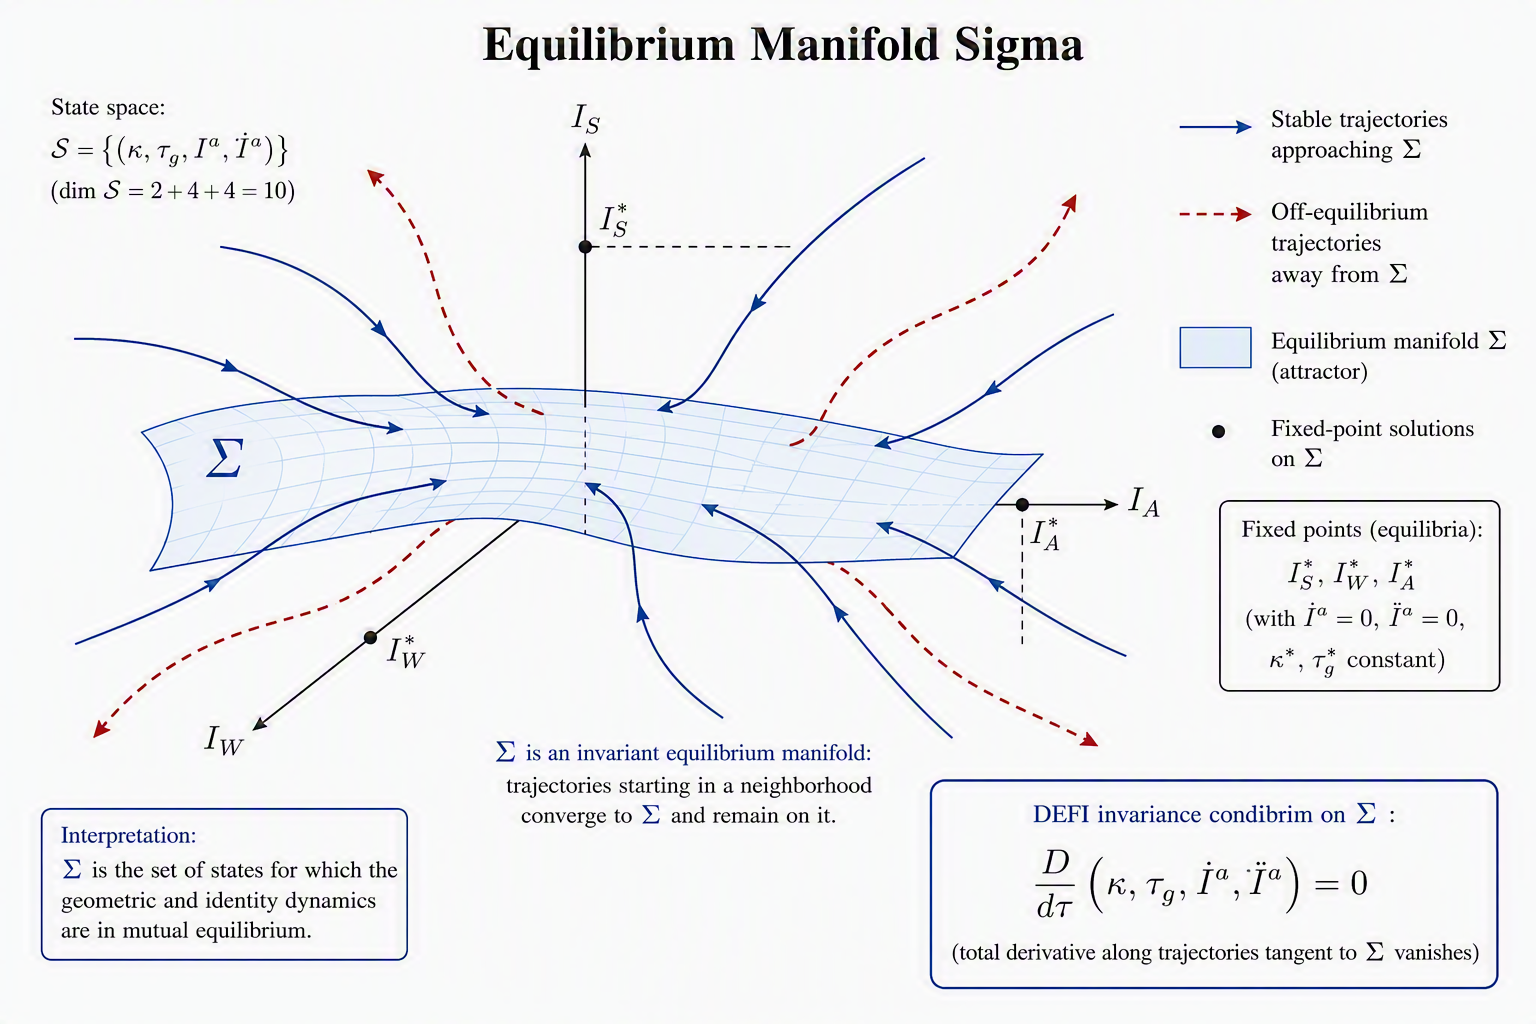
\includegraphics[width=0.95\textwidth]{fig4_equilibrium_sigma.jpg}
 \caption{ Equilibrium manifold $\Sigma$ defined by the fixed-point conditions of the coupled DEFI equations. Stable trajectories converge toward the manifold, while off-equilibrium trajectories move away from it. }
 \label{fig:equilibrium_sigma}
 \end{figure}

A fixed point of the coupled system is a configuration at which every identity
acceleration vanishes, $\ddot I_S=\ddot I_W=\ddot I_A=0$, so that the identity
sector is at rest relative to the instantaneous geometry $(\kappa,\tau_g)$. Note
that this is \emph{not} the same as setting $\partial U_{\text{DEFI}}/\partial
I^a=0$: the harmonic terms of $L_{\text{ident}}$ contribute to each equation of
motion alongside $U_{\text{DEFI}}$, so the fixed point must be read off the full
equations of motion of Sec.~IV rather than from $U_{\text{DEFI}}$ alone. Setting
the left-hand sides of those equations to zero gives the fixed-point values
explicitly, as functions of the instantaneous geometry:
\begin{align}
I_S^\ast(\kappa,I_A) &= -\frac{\mu_1(I_A)}{\gamma}\,\kappa^2,
\label{eq:fixedS}\\
I_W^\ast(\tau_g,I_A) &= -\frac{\mu_2(I_A)}{\delta}\,\tau_g^2,
\label{eq:fixedW}\\
0 &= \mu_1'(I_A)\,\kappa^2 I_S^\ast + \mu_2'(I_A)\,\tau_g^2 I_W^\ast + \beta I_A,
\label{eq:fixedA}
\end{align}
with Eq.~\eqref{eq:fixedA} an implicit equation fixing $I_A^\ast(\kappa,\tau_g)$
once Eqs.~\eqref{eq:fixedS}--\eqref{eq:fixedW} are substituted in. At any point
$(\kappa,\tau_g,I_A^\ast,I_S^\ast,I_W^\ast)$ satisfying
Eqs.~\eqref{eq:fixedS}--\eqref{eq:fixedA} simultaneously, the identity
accelerations vanish identically and the geometric equations of motion decouple
from the identity sector at that instant. This is exactly
\begin{equation}
\frac{D}{d\tau}\left(\kappa,\ \tau_g,\ \dot I^a,\ \ddot I^a\right) = 0,
\end{equation}
i.e., Eq.~\eqref{eq:stipulated}, now characterized as the fixed-point condition
of the DEFI action rather than an axiom. The stability manifold $\Sigma$ of the
unified paper \cite{DuttonUnified2026} is precisely the graph of
Eqs.~\eqref{eq:fixedS}--\eqref{eq:fixedA} in $M\times\mathcal{I}$ — the locus
where the identity sector has relaxed onto the geometry it is coupled to — and
the previously stipulated condition follows from Eq.~\eqref{eq:action} rather
than defining it. Off this locus, Eqs.~\eqref{eq:fixedS}--\eqref{eq:fixedA} fail
to hold, $\ddot I^a\neq0$, and the identity sector is out of equilibrium with the
geometry, exactly as required for $\Sigma$ to be a nontrivial proper subset of
$M\times\mathcal{I}$ rather than the whole configuration space.

\section{Conserved Origin Charge}
\label{sec:origin}

Because $I_O$ does not appear in $U_{\text{DEFI}}$, the Origin sector is fully
decoupled: its equation of motion,
\begin{equation}
\ddot I_O = -I_O,
\end{equation}
depends on no other variable in the theory. The Origin sector's own energy
function,
\begin{equation}
Q_O = \frac{1}{2}\alpha\left(\dot I_O^{\,2} + I_O^2\right),
\end{equation}
satisfies $\dot Q_O = \dot I_O\left(\alpha \ddot I_O + \alpha I_O\right) = 0$
identically along the Origin equation of motion, independent of the state of the
geometry or the other identity coordinates. This is the Noether charge
\cite{Noether1918,Noether1971} associated
with the $\tau$-translation symmetry restricted to the autonomous Origin
subsystem: because $L_\text{ident}$ contains no cross term coupling $I_O$ to
$(I_A,I_S,I_W,\kappa,\tau_g)$, the O-sector's own Hamiltonian is separately
conserved even though it sits inside a larger interacting system. $Q_O$ is
therefore a genuine conserved quantity, not merely an initial condition — Origin
is both where the trajectory starts and an invariant preserved throughout its
evolution, consistent with its intended role as the foundational, unchanging
layer of SEFI identity \cite{DuttonSEFI2026}.

\section{Relation to GWFM, SEFI, and the Unified Theory}

\begin{itemize}
\item \textbf{GWFM limit.} Setting $I^a=$ const (identity frozen) removes all
coupling; $S_{\text{DEFI}}\to \int L_{\text{geom}}\,d\tau$, recovering pure GWFM
worldline dynamics \cite{DuttonElectronField2026}.
\item \textbf{SEFI limit.} Setting $\kappa=\tau_g=0$ (a straight, torsion-free
worldline) removes the coupling term entirely; $S_{\text{DEFI}}\to\int
L_{\text{ident}}\,d\tau$, recovering the identity-space dynamics of SEFI under
Axiom 0's vectorization, with the original scalar $F$ recovered by contraction
(Sec.~1.1).
\item \textbf{Unified operator.} The potentials $V_{\text{geom}}, V_{\text{ident}},
V_{\text{dyn}}$ of the unified transformation operator $T$
\cite{DuttonUnified2026} correspond respectively to the $\kappa^2,\tau_g^2$ terms
of $L_{\text{geom}}$'s curvature expansion, the quadratic terms of
$L_{\text{ident}}$, and $U_{\text{DEFI}}$ of Eq.~\eqref{eq:coupling}. This
construction therefore supplies the variational principle the unified paper's
Limitations section identifies as missing.
\end{itemize}

\section{Limitations and Future Work}

The coupling potential~\eqref{eq:coupling} is the simplest form consistent with
the qualitative SEFI canon and full two-way symmetry; it is not derived from a
deeper principle and other bilinear forms are equally consistent with the
stated constraints. The functions $\mu_1(I_A),\mu_2(I_A)$ are unconstrained by
the present construction beyond differentiability. Stability of the fixed-point
locus $\Sigma$ defined by Eqs.~\eqref{eq:fixedS}--\eqref{eq:fixedA} (linear
stability of the coupled equations about that locus, in the sense standard to
coupled-oscillator and dynamical-systems analysis \cite{Strogatz2015}) has not
been analyzed and
is needed before $\Sigma$ can be asserted to be attracting rather than merely
stationary. Quantization of $S_{\text{DEFI}}$, and its compatibility with the
eigenvalue problem $T\Psi_n=\lambda_n\Psi_n$ of the unified operator, is left to
future work.

\section{Conclusion}

DEFI has been constructed as a coupled Lagrangian dynamical system on
$M\times\mathcal{I}$, with a fully symmetric coupling potential linking GWFM
curvature/torsion to SEFI's Sovereignty and Warp identity coordinates, weighted
by Authorship. The previously stipulated dynamical invariance condition is
recovered as an equilibrium condition of this system rather than assumed, and a
conserved Origin charge has been derived via Noether's theorem for the decoupled
Origin sector. This construction required an explicit, stated extension of SEFI's
scalar identity functional to a four-vector, recorded here as Axiom 0 rather than
left implicit.

\begin{thebibliography}{9}

\bibitem{DuttonSEFI2026}
J. Dutton, \emph{SEFI: The Single Entity Field Interpretation --- Formal
Mathematical Construction}, 2026.

\bibitem{DuttonElectronField2026}
J. Dutton, \emph{Geometric Worldline Foundations of the Electron Field}, 2026.

\bibitem{DuttonUnified2026}
J. Dutton, \emph{Unified Geometric Field Theory from Worldline and
Identity-Space Invariants}, 2026.

\bibitem{GoldsteinPooleSafko2002}
H. Goldstein, C. P. Poole, and J. L. Safko, \emph{Classical Mechanics}, 3rd ed.
(Addison-Wesley, 2002).

\bibitem{Noether1918}
E. Noether, ``Invariante Variationsprobleme,'' Nachr. Ges. Wiss. G\"ottingen,
Math-phys. Klasse, 235--257 (1918).

\bibitem{Noether1971}
E. Noether, ``Invariant Variation Problems,'' trans. M. A. Tavel,
\emph{Transport Theory and Statistical Physics} \textbf{1}, 183--207 (1971).

\bibitem{DoCarmo1976}
M. P. do Carmo, \emph{Differential Geometry of Curves and Surfaces}
(Prentice-Hall, 1976).

\bibitem{MarsdenRatiu1999}
J. E. Marsden and T. S. Ratiu, \emph{Introduction to Mechanics and Symmetry},
2nd ed. (Springer, 1999).

\bibitem{Strogatz2015}
S. H. Strogatz, \emph{Nonlinear Dynamics and Chaos}, 2nd ed. (Westview Press,
2015).

\end{thebibliography}

\end{document}
